%%%%%%%%%%%%%%%%%%%%%%%%
% Results and Analysis | Chapter 4
%%%%%%%%%%%%%%%%%%%%%%%%
\chapter{Results and Analysis}
\label{chp:results}

\section{RQ1.1. To what extent can generative AI improve the usability of a UI?}
\subsection{Visualisation of the data}
\subsection{Answer to the research question}
Snacka lite om interjuverna detta med att AI hjälper med Uiet:
Ta upp om att man kan kolla om man är på rätt spår (får smama svar som AI / man kollar på samma data)

\section{RQ1.2. What are the key challenges for users using generative AI for data visualization in web applications?}
\subsection{Visualisation of the data}
\subsection{Answer to the research question}

\section{RQ1.3: Can generative AI help to improve perceived efficiency and task completion when working with a data-intensive web application?}
\subsection{Visualisation of the data}
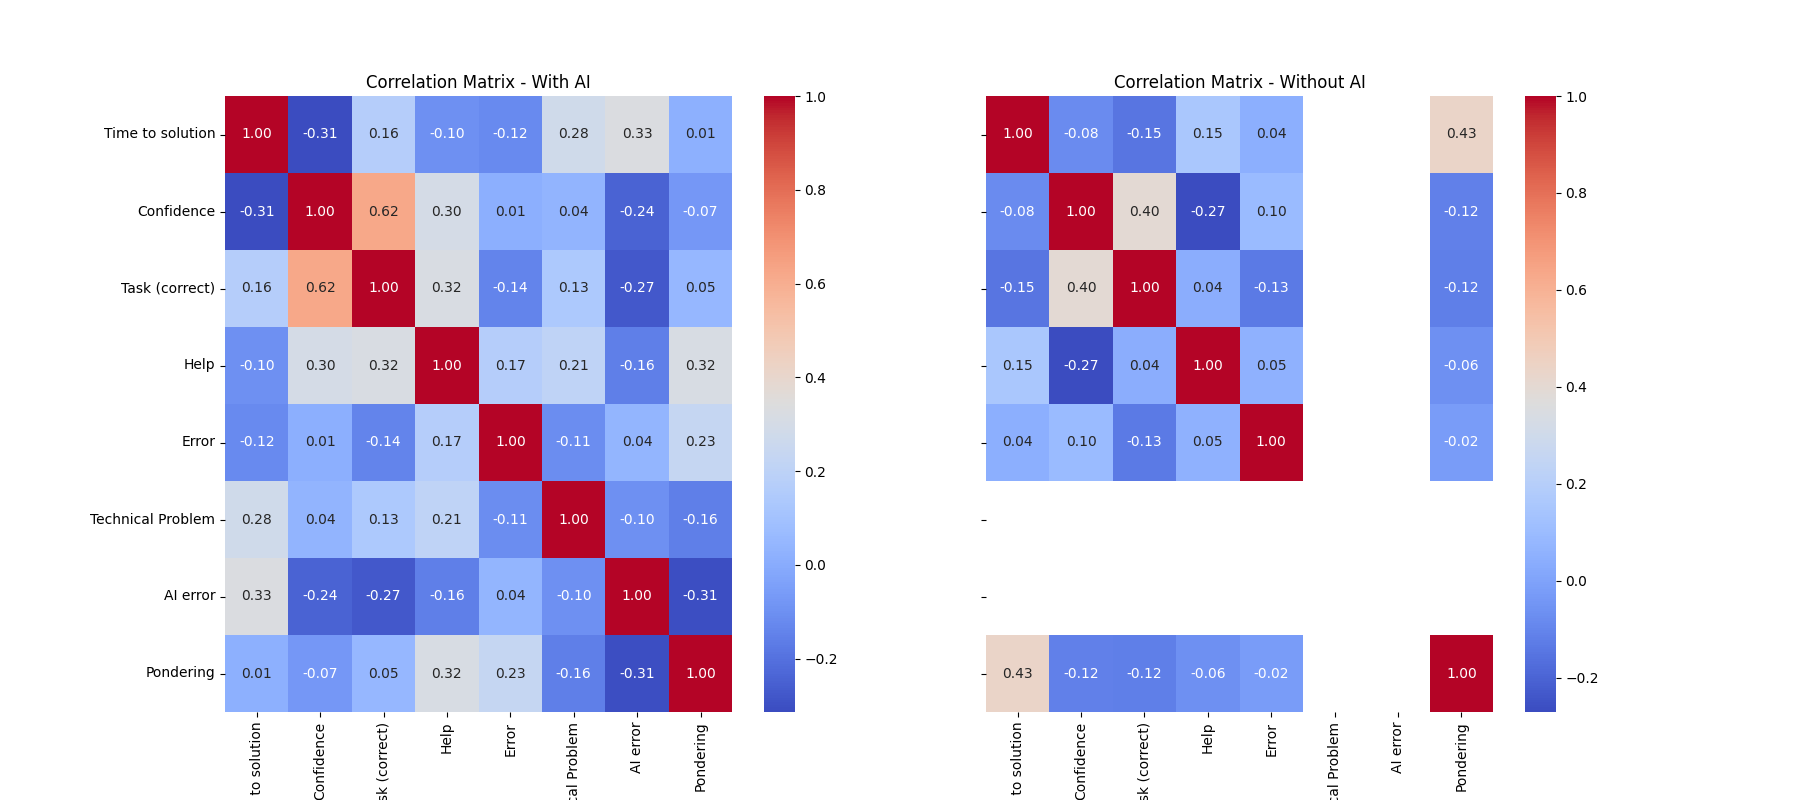
\includegraphics[width=\textwidth]{Images/correlation_matrix_split_treatment.png}
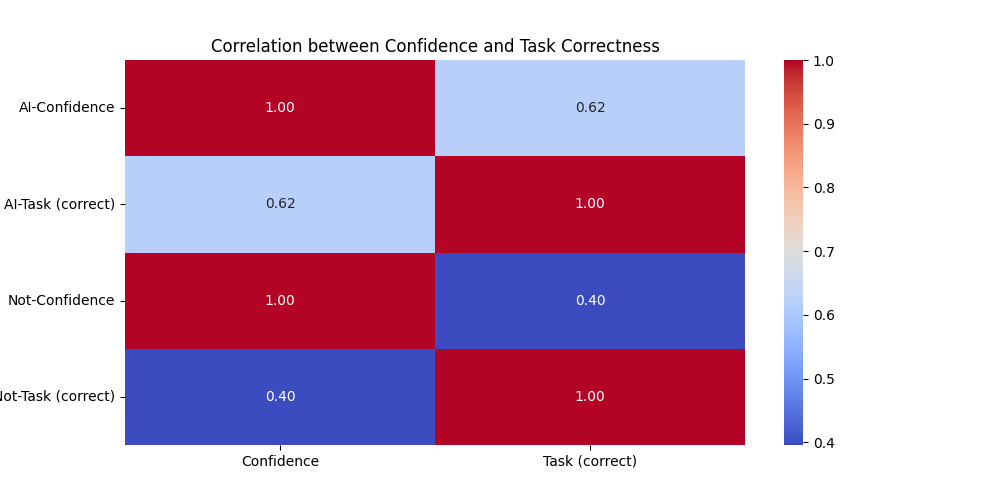
\includegraphics[width=\textwidth]{Images/confidence_correlation_heatmap.png}
 - Confidence in task results seem to correlate more with actual results when using AI.
 - Generally slower results produced, atleast in a small scale like this.
 - Accuracy in answers are also lower when using AI.
 - The slower and less accurate results probably has more to do with the implementation of the AI itself rather than the usage AI could possibly have in data intensive applications.
\subsection{Answer to the research question}

\section{RQ1. Can the use of generative AI help improve the user experience in a data-intensive web application compared to traditional user interface methods?}
\subsection{Visualisation of the data}
\subsection{Answer to the research question}
